%%%%%%%%%%%%%%%%%%%%%%%%%%%%%%%%%%%%%%%%%%%%%%%%%%%%%%%%%%%%%%%%%%%%%%%%%%%%%%%%
%% CSC B63 -- Example use of LaTeX to typeset assignment solutions
%%%%%%%%%%%%%%%%%%%%%%%%%%%%%%%%%%%%%%%%%%%%%%%%%%%%%%%%%%%%%%%%%%%%%%%%%%%%%%%%

\documentclass[fleqn]{article}

\usepackage{amsmath,amssymb,amsthm}
\usepackage{upquote}
\usepackage{hyperref}
\usepackage{tikz}
\usepackage{forest}
\usepackage{geometry}
\usetikzlibrary{graphs}

% shortcuts for things commonly used in our class:
\newcommand{\code}{\texttt}
\newcommand{\nat}{\mathbb{N}}
\newcommand{\real}{\mathbb{R}}
\newcommand{\realp}{\mathbb{R}^+}
\newcommand{\bigo}[1]{\mathcal{O}(#1)}

% command to allow page breaks in align and similar environments
\newcommand{\br}{\displaybreak[0] \\}

% character in a cirle, good to refer to nodes
\newcommand*\circled[1]{\tikz[baseline=(char.base)]{
            \node[shape=circle,draw,inner sep=2pt] (char) {#1};}}

\theoremstyle{definition}  % I don't like italics


\begin{document}

\section{Getting Started}

Overleaf (\href{https://www.overleaf.com}{https://www.overleaf.com}) is a great place to start. It is
a web-based WYSIWYG (what-you-see-is-what-you-get) environment, and it provides some very useful
tutorials.

\section{Math stuff}

Here's the source for the first question on your assignment 1: \bigskip

Prove each of the following {\em using the definitions of } Big-Oh / Big-Omega / Big-Theta.

\begin{itemize}
\item If $f \in \bigo{g}$ and $g \in \bigo{h}$ then $f \in \bigo{h}$, for all functions $f$, $g$,
  $h$ in $\nat \to \realp$.

\item If $f_1 \in \bigo{g_1}$ and $f_2 \in \bigo{g_2}$ then $f \in \bigo{g}$, where
  $f(n) = f_1(n) \cdot f_2(n)$, $g(n) = g_1(n) \cdot g_2(n)$, for all functions $f_1$, $f_2$, $g_1$,
  $g_2$ in $\nat \to \realp$.

\item $2^{2n} \not\in \bigo{2^n}$.

\item If $f_1 \in \bigo{g}$ and $f_2 \in \bigo{g}$ then $f_{\max} \in \bigo{g}$, where $f_{\max}$ is
  defined by $f_{\max}(n) = \max(f_1(n), f_2(n))$, for all functions $f_1$, $f_2$, $g$ in
  $\nat \to \realp$.
\end{itemize}

If we wanted a numbered list, we would have used the \textbf{enumerate} environment:

\begin{enumerate}
\item If $f \in \bigo{g}$ and $g \in \bigo{h}$ then $f \in \bigo{h}$, for all functions $f$, $g$, $h$ in $\nat \to \realp$.

\item $\hdots$

\end{enumerate}

\section{Proof stuff}

Here's one way to structure a proof:

\newtheorem{lem}{Lemma}
\begin{lem}
  What to prove goes here.
\end{lem}
\begin{proof}
  And the proof goes here.
\end{proof}

\begin{lem}
  What to prove goes here.
\end{lem}
\begin{proof}
  And the proof goes here.
\end{proof}

\newtheorem{thm}{Theorem}
\begin{thm}
  What to prove goes here.
\end{thm}
\begin{proof}
  And the proof goes here.
\end{proof}


\section{Trees and Graphs}

My favourite way to draw a tree quickly:

\begin{center}
  \begin{forest}
    for tree={circle, draw, s sep=10mm, inner sep=1pt, minimum size=5pt}
    [10
    [9 [3] [,phantom]]
    [19 [14 [12] [,phantom]]
    [34 [20] [37]]]]
  \end{forest}
\end{center}

A longer, but super flexible and customizable way:
    \begin{center}
      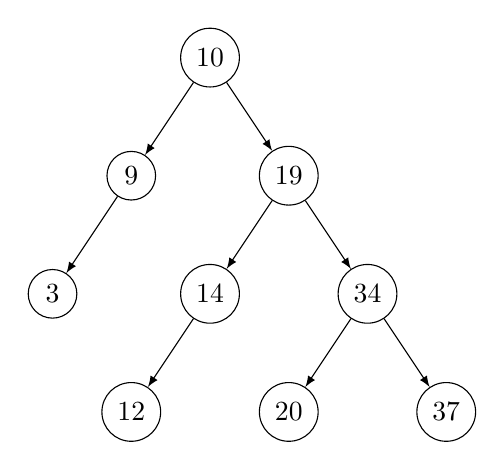
\begin{tikzpicture}
        \draw[level distance=15mm, level/.style={sibling distance=20mm}, every node/.style={circle,draw},
              edge from parent/.style={-latex,draw}, font=\rmfamily]
        node{10}
        child{node{9}
          child{node{3}}
          child[missing]
        }
        child{node{19}
          child{node{14}
            child{node{12}}
            child[missing]}
          child{node{34}
            child{node{20}}
            child{node{37}}}
        };
      \end{tikzpicture}
    \end{center}

    Here's a graph:

    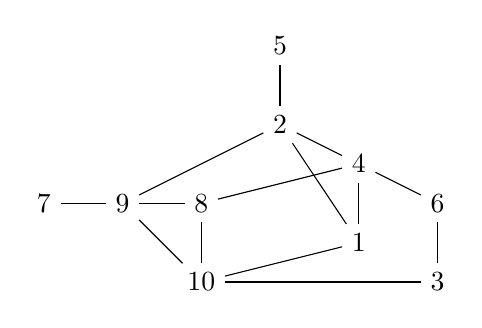
\begin{tikzpicture}
      \node (5) at (3,0) {5};
      \node (2) at (3,-1) {2};
      \node (7) at (0,-2) {7};
      \node (9) at (1,-2) {9};
      \node (8) at (2,-2) {8};
      \node (4) at (4,-1.5) {4};
      \node (1) at (4,-2.5) {1};
      \node (6) at (5,-2) {6};
      \node (10) at (2,-3) {10};
      \node (3) at (5,-3) {3};

      \graph{
        (1) -- (2);
        (1) -- (4);
        (1) -- (10);
        (2) -- (4);
        (2) -- (5);
        (2) -- (9);
        (3) -- (6);
        (3) -- (10);
        (4) -- (6);
        (4) -- (8);
        (7) -- (9);
        (8) -- (9);
        (8) -- (10);
        (9) -- (10)
      };
    \end{tikzpicture}
    \newpage

    And a more complicated graph:

    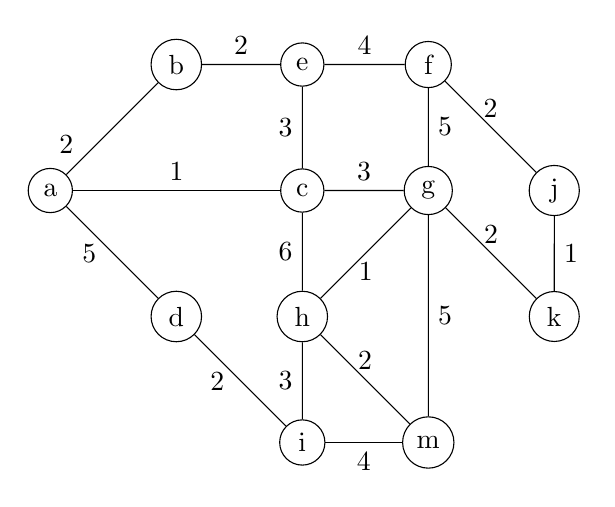
\begin{tikzpicture}[scale=0.8]
      \node[draw,circle] (a) at (0,4) {a};
      \node[draw,circle] (b) at (2,6) {b};
      \node[draw,circle] (c) at (4,4) {c};
      \node[draw,circle] (d) at (2,2) {d};
      \node[draw,circle] (e) at (4,6) {e};
      \node[draw,circle] (f) at (6,6) {f};
      \node[draw,circle] (g) at (6,4) {g};
      \node[draw,circle] (h) at (4,2) {h};
      \node[draw,circle] (i) at (4,0) {i};
      \node[draw,circle] (j) at (8,4) {j};
      \node[draw,circle] (k) at (8,2) {k};
      \node[draw,circle] (m) at (6,0) {m};

      \draw (a) -- (b) node [at start, above=4pt] {2};
      \draw (a) -- (c) node [midway, above] {1};
      \draw (a) -- (d) node [near start, below=2pt] {5};
      \draw (b) -- (e) node [midway, above] {2};
      \draw (c) -- (e) node [midway, left] {3};
      \draw (c) -- (g) node [midway, above] {3};
      \draw (c) -- (h) node [midway, left] {6};
      \draw (d) -- (i) node [near start, below=2pt] {2};
      \draw (e) -- (f) node [midway, above] {4};
      \draw (f) -- (g) node [midway, right] {5};
      \draw (f) -- (j) node [midway, above] {2};
      \draw (g) -- (h) node [midway, below] {1};
      \draw (g) -- (m) node [midway, right] {5};
      \draw (g) -- (k) node [midway, above] {2};
      \draw (h) -- (m) node [midway, above] {2};
      \draw (h) -- (i) node [midway, left] {3};
      \draw (i) -- (m) node [midway, below] {4};
      \draw (j) -- (k) node [midway, right] {1};
    \end{tikzpicture}


\end{document}
